As dimensões de átomos, íons e comprimentos de ligação situam-se na faixa de 10-10 m, que equivale 1 \AA (ângstron) ou 100 pm (picômetro). Por exemplo, o raio covalente do hidrogênio é de 74 pm. Suponha que os átomos de hidrogênio possam ser dispostos lado a lado em uma única linha, conforme sugerido no diagrama abaixo:

\begin{center}
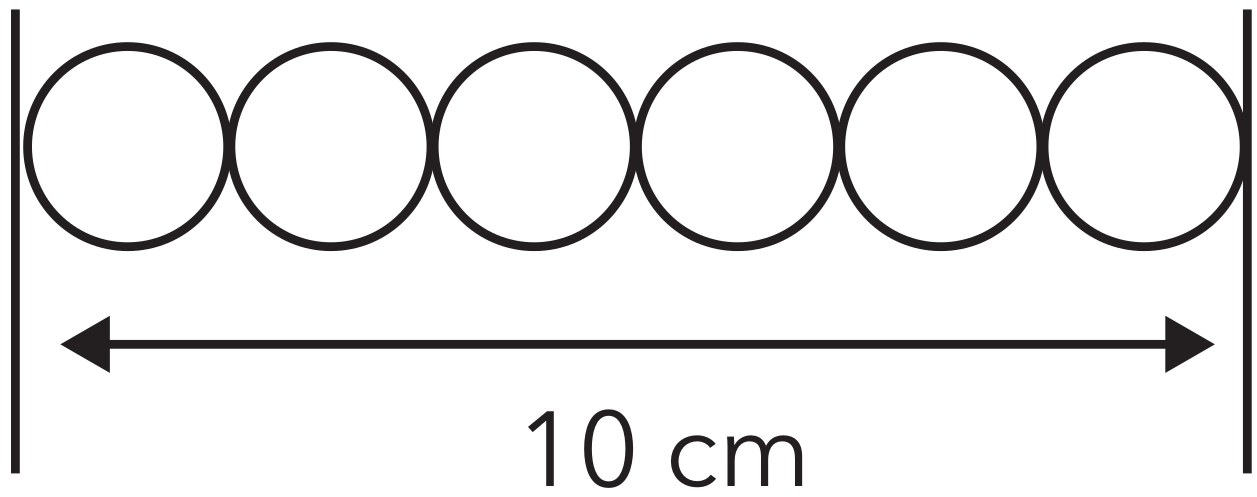
\includegraphics[width=0.25\textwidth]{figure.png}
\end{center}

\begin{enumerate}[label = (\alph*)]
	\item $7,4 \times 10^{-11}$
	\item $7,4 \times 10^{-10}$
	\item $2,3 \times 10^{-15}$
	\item $1,1 \times 10^{-21}$
	\item $1,1 \times 10^{-15}$
\end{enumerate}
